\documentclass[11pt,oneside]{book}
\usepackage[T1]{fontenc}
%\usepackage[utf8]{inputenc}
\usepackage[a4paper]{geometry}
\usepackage[sectionbib]{natbib}
\usepackage{chapterbib}
\usepackage{graphicx}
\usepackage{hyperref}
%%% Uncomment if you change the bibliography heading/title
% \renewcommand{\bibname}{References}

%%% Uncomment if you want to include the bibliographies at the end of each chapter in the table of contents.  
% \usepackage[nottoc]{tocbibind}


%%%%%%%%%%%%%%%%%%%%%%%%%%%%%%%%%%%%%%%%%%%%%%%%%%%%%%%%%%%%%%%%%%%%%%%%%%%%%%%%
% 'dedication' environment: To add a dedication paragraph at the start of book %
% Source: http://www.tug.org/pipermail/texhax/2010-June/015184.html            %
%%%%%%%%%%%%%%%%%%%%%%%%%%%%%%%%%%%%%%%%%%%%%%%%%%%%%%%%%%%%%%%%%%%%%%%%%%%%%%%%
\newenvironment{dedication}
{
   \cleardoublepage
   \thispagestyle{empty}
   \vspace*{\stretch{1}}
   \hfill\begin{minipage}[t]{0.66\textwidth}
   \raggedright
}
{
   \end{minipage}
   \vspace*{\stretch{3}}
   \clearpage
}


%%%%%%%%%%%%%%%%%%%%%%%%%%%%%%%%%%%%%%%%%%%%%%%%
% Chapter quote at the start of chapter        %
% Source: http://tex.stackexchange.com/a/53380 %
%%%%%%%%%%%%%%%%%%%%%%%%%%%%%%%%%%%%%%%%%%%%%%%%
\makeatletter
\renewcommand{\@chapapp}{}% Not necessary...
\newenvironment{chapquote}[2][2em]
  {\setlength{\@tempdima}{#1}%
   \def\chapquote@author{#2}%
   \parshape 1 \@tempdima \dimexpr\textwidth-2\@tempdima\relax%
   \itshape}
  {\par\normalfont\hfill--\ \chapquote@author\hspace*{\@tempdima}\par\bigskip}
\makeatother


%%%%%%%%%%%%%%%%%%%%%%%%%%%%%%%%%%%%%%%%%%%%%%%%%%%%%%%%%%%%%%%%%%%%%%%%%%%%%%%%
% calchub environment: for embedding a calchub workspace                       %
% texedbook compatible: html=embedded work space, pdf=multimedia box w/ href   %
%%%%%%%%%%%%%%%%%%%%%%%%%%%%%%%%%%%%%%%%%%%%%%%%%%%%%%%%%%%%%%%%%%%%%%%%%%%%%%%%
\newenvironment{calchub}
    {\begin{center}
    \begin{tabular}{|p{0.9\textwidth}|}
    \hline
    Multimedia content: CalcHub Workspace\\
    \hline\\
    }
    { 
    \\\\\hline
    \end{tabular} 
    \end{center}
    }

\newcommand{\InsertCalchubWorkspace}[2]{ 
   % 1st input: display name 
   % 2nd input: href
   \begin{calchub}
      \href{#2}{#1}
   \end{calchub}
} 


%%%%%%%%%%%%%%%%%%%%%%%%%%%%%%%%%%%%%%%%%%%%%%%%%%%%%%%%%%%%%%%%%%%%%%%%%%%%%%%%
% video environment: for embedding videos                                      %
% texedbook compatible: html=embedded video, pdf=multimedia box w/ href        %
%%%%%%%%%%%%%%%%%%%%%%%%%%%%%%%%%%%%%%%%%%%%%%%%%%%%%%%%%%%%%%%%%%%%%%%%%%%%%%%%
\newenvironment{youtube}
    {\begin{center}
    \begin{tabular}{|p{0.9\textwidth}|}
    \hline
    Multimedia content: YouTube Video\\
    \hline\\
    }
    { 
    \\\\\hline
    \end{tabular} 
    \end{center}
    }

\newcommand{\InsertYoutubeVideo}[2]{ 
   % 1st input: display name 
   % 2nd input: href
   \begin{youtube}
      \href{#2}{#1}
   \end{youtube}
} 


%%%%%%%%%%%%%%
% Title Page %
%%%%%%%%%%%%%%

% Book's title and subtitle
\title{\Huge \textbf{Texedbook}}
% Authors
\author{\textsc{Riley Hanus}}

\begin{document}
\frontmatter
\maketitle

\chapter*{Abstract}
This is \emph{not} a full thesis template! It only demonstrates how to create per-chapter references using the \texttt{chapterbib} package with BibTeX. (Do not use with BibLaTeX!)

Each chapter must be in its own \texttt{.tex} file and \texttt{include}-d into the main \texttt{.tex} file. If compiling on your own machine, run \texttt{bibtex} on \emph{each} generated \texttt{.aux} file, before running \texttt{pdflatex} twice more. (These are done automatically on Overleaf.)

\tableofcontents

\mainmatter
\chapter{First Test Chapter}

\begin{chapquote}{Author's name, \textit{Source of this quote}}
    ``This is a quote and I don't know who said this.''
\end{chapquote}
    
\section{Lists}
Lorem ipsum dolor sit amet \citep{Ohno2007}, consectetur adipisicing elit, sed do eiusmod tempor incididunt ut labore et dolore magna aliqua.

Ut enim ad minim veniam, quis nostrud exercitation ullamco laboris nisi ut aliquip ex ea commodo consequat. 

\subsection{Numbered list}
Duis aute irure dolor in reprehenderit in voluptate velit esse cillum dolore eu fugiat nulla pariatur. Excepteur sint occaecat cupidatat non proident, sunt in culpa qui officia deserunt mollit anim id est laborum. \\ Lorem ipsum list:

1. Lorem ipsum dolor sit amet, consectetur adipiscing elit.

2. Duis ac mi magna, a consectetur elit.

3. Curabitur posuere erat \emph{dignissim ligula euismod} ut euismod nisi.

4. Fusce vulputate facilisis neque, et ornare mauris mattis vel.

5. Mauris sit amet nulla mi, vitae rutrum ante.

6. Maecenas quis nulla risus, vel tincidunt ligula.

7. Nullam ac enim neque, non \emph{dapibus} mauris.

8. Integer volutpat leo a orci suscipit eget rhoncus urna eleifend.

\noindent Lorem ipsum dolor sit amet, consectetur adipiscing elit. Duis risus ante, auctor et pulvinar non, posuere ac lacus. Praesent egestas nisi id metus rhoncus ac lobortis sem hendrerit. Etiam et sapien eget lectus interdum posuere sit amet ac urna:

\subsection{Bulleted list}
Lorem ipsum dolor sit amet, consectetur adipiscing elit. Duis risus ante, auctor et pulvinar non, posuere ac lacus. Praesent egestas nisi id metus rhoncus ac lobortis sem hendrerit. Etiam et sapien eget lectus interdum posuere sit amet ac urna. Aliquam pellentesque imperdiet erat, eget consectetur felis malesuada quis. Pellentesque sollicitudin, odio sed dapibus eleifend, magna sem luctus turpis, id aliquam felis dolor eu diam. Etiam ullamcorper, nunc a accumsan adipiscing, turpis odio bibendum erat, id convallis magna eros nec metus. Sed vel ligula justo, sit amet vestibulum dolor. Sed vitae augue sit amet magna ullamcorper suscipit. Quisque dictum ipsum a sapien egestas facilisis. \\ Lorem ipsum list:
\begin{itemize}
\item Mauris sit amet nulla mi, vitae rutrum ante.
\item Maecenas quis nulla risus, vel tincidunt ligula.
\item Nullam ac enim neque, non \emph{dapibus} mauris.
\end{itemize}

\section{Table}
Lorem ipsum dolor sit amet, consectetur adipisicing elit, sed do eiusmod tempor incididunt ut labore et dolore magna aliqua. Ut enim ad minim veniam, quis nostrud exercitation ullamco laboris nisi ut aliquip ex ea commodo consequat.

%%%%%%%%%%%%%%%%%%%%%%%%%%%%%%%%%%%%%%%%%%%%%%%%%%%%%%%
% Sample table                                        %
% Source: www1.maths.leeds.ac.uk/latex/TableHelp1.pdf %
%%%%%%%%%%%%%%%%%%%%%%%%%%%%%%%%%%%%%%%%%%%%%%%%%%%%%%%
\begin{table}[ht]
\caption{Sample table} % title of Table
\centering % used for centering table
\begin{tabular}{c c c c}
% centered columns (4 columns)
\hline\hline %inserts double horizontal lines
S. No. & Column\#1 & Thermal conductivity, $\kappa_\mathrm{pg}$ & Column\#3 \\ [0.5ex]
% inserts table
%heading
\hline % inserts single horizontal line
1 & 50 & 837 & 970 \\
2 & 47 & 877 & 230 \\
3 & 31 & 25 & 415 \\
4 & 35 & 144 & 2356 \\
5 & 45 & 300 & 556 \\ [1ex] % [1ex] adds vertical space
\hline %inserts single line
\end{tabular}
\label{table:nonlin} % is used to refer this table in the text
\end{table}

Duis aute irure dolor in reprehenderit in voluptate velit esse cillum dolore eu fugiat nulla pariatur. Excepteur sint occaecat cupidatat non proident, sunt in culpa qui officia deserunt mollit anim id est laborum. 

\section{Custom functions}
Lorem ipsum dolor sit amet, consectetur adipisicing elit, sed do eiusmod tempor incididunt ut labore et dolore magna aliqua.

Ut enim ad minim veniam, quis nostrud exercitation ullamco laboris nisi ut aliquip ex ea commodo consequat.

\subsection{YouTube}

\InsertYoutubeVideo{Fourier Transforms}{https://www.youtube.com/watch?v=r6sGWTCMz2k}
% \InsertYoutubeVideo{Calculus}{https://www.youtube.com/watch?v=WUvTyaaNkzM}

\subsection{CalcHub}

Duis aute irure dolor in reprehenderit in voluptate velit esse cillum dolore eu fugiat nulla pariatur. Excepteur sint occaecat cupidatat non proident, sunt in culpa qui officia deserunt mollit anim id est laborum. 

\InsertCalchubWorkspace{Sample CalcHub Workspace}{https://calchub.co/calcs/16c5e5ef}

Duis aute irure dolor in reprehenderit in voluptate velit esse cillum dolore eu fugiat nulla pariatur. Excepteur sint occaecat cupidatat non proident, sunt in culpa qui officia deserunt mollit anim id est laborum. 

\InsertCalchubWorkspace{Sample CalcHub Workspace}{https://calchub.co/calcs/16c5e5ef}


%\bibliographystyle{unsrtnat}  %% For numerical citations remember to pass "numbers" option to natbib
\bibliographystyle{unsrt}
\bibliography{sample}
\chapter{Equations and Figures }

\section{Equations}
Lorem ipsum dolor sit amet, $\kappa_\mathrm{pg}$
consectetur adipiscing elit. Duis risus ante, auctor et pulvinar non, posuere ac lacus. Praesent egestas nisi id metus rhoncus ac lobortis sem hendrerit Eq. \mjref{eq:Callaway}. Etiam et sapien eget lectus interdum posuere sit amet ac urna. Aliquam pellentesque imperdiet erat, eget consectetur felis malesuada quis. Pellentesque sollicitudin, odio sed dapibus eleifend, magna sem luctus turpis, id aliquam felis dolor eu diam. Etiam ullamcorper, nunc a accumsan adipiscing, turpis odio bibendum erat, id convallis magna eros nec metus. Sed vel ligula justo, sit amet vestibulum dolor. Sed vitae augue sit amet magna ullamcorper suscipit. Quisque dictum ipsum a sapien egestas facilisis.

\begin{equation}
  \kappa_\mathrm{pg}=\frac{1}{3} \intop _0 ^{\omega_\mathrm{max}} C(\omega) \, v_\mathrm{g}(\omega)^2 \, \tau(\omega) \, d\omega. \label{eq:Callaway}
\end{equation}

Test. Etiam ullamcorper, nunc a accumsan adipiscing, turpis odio bibendum erat, id convallis magna eros nec metus. Sed vel ligula justo, sit amet vestibulum dolor. Sed vitae augue sit amet magna ullamcorper suscipit. Quisque dictum ipsum a sapien egestas facilisis. 

\section{Figure}
\noindent Lorem ipsum dolor sit amet Figure \ref{fig:test}, consectetur adipiscing elit. Reference something in Chapter 1, Table \ref{table:nonlin}. Duis risus ante, auctor et pulvinar non, posuere ac lacus. Praesent egestas nisi id metus rhoncus ac lobortis sem hendrerit. Etiam et sapien eget lectus interdum posuere sit amet ac urna \citep{latex:companion}. Etiam et sapien eget lectus interdum posuere sit amet ac urna. Aliquam pellentesque imperdiet erat, eget consectetur felis malesuada quis. Pellentesque sollicitudin, odio sed dapibus eleifend, magna sem luctus turpis, id aliquam felis dolor eu diam. Etiam ullamcorper, nunc a accumsan adipiscing, turpis odio bibendum erat, id convallis magna eros nec metus. Sed vel ligula justo, sit amet vestibulum dolor. Sed vitae augue sit amet magna ullamcorper suscipit. Quisque dictum ipsum a sapien egestas facilisis. \href{http://thermoelectrics.matsci.northwestern.edu/}{Snyder's thermoelectrics website.}

\begin{figure}
  \centering
  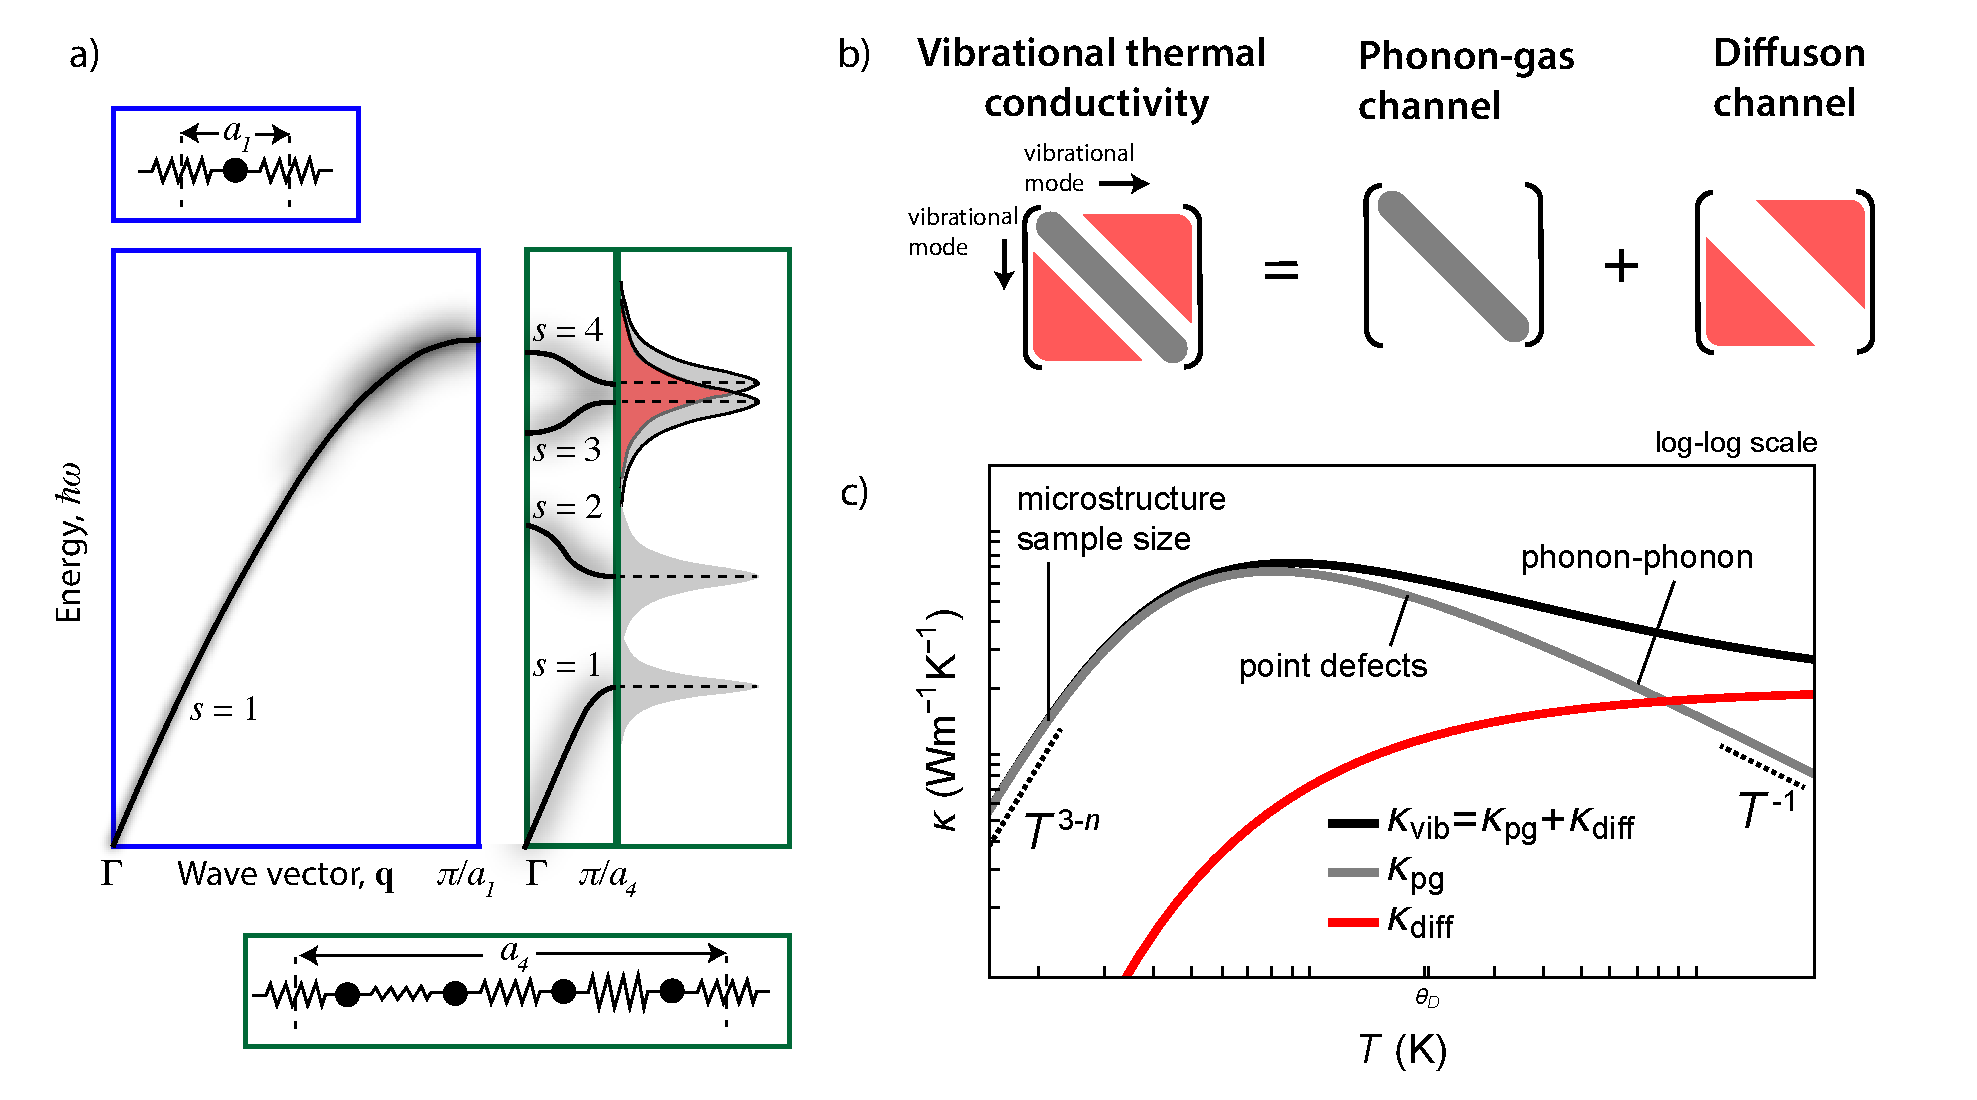
\includegraphics[width=0.99\textwidth, keepaspectratio]{test-fig.pdf}
  \caption{Figure Lorem ipsum dolor sit amet, consectetur adipiscing elit. Duis risus ante, auctor et pulvinar non, posuere ac lacus. Praesent egestas nisi id metus rhoncus ac lobortis sem hendrerit.}
  \label{fig:test}
\end{figure}

%\bibliographystyle{unsrtnat}  %% For numerical citations remember to pass "numbers" option to natbib
\bibliographystyle{unsrt}
\bibliography{sample}


\backmatter
\chapter*{Afterword}
%\addcontentsline{toc}{chapter}{Additional Reading}
\nocite{lim:etal:kdtei:2016,markdown:overleaf}   % .bib keys of your own publications

{\renewcommand{\bibsection}{}
\bibliographystyle{dcu}
\bibliography{sample}
}

\end{document}
